\documentclass[10pt]{beamer}

\usetheme{metropolis}
\usepackage{appendixnumberbeamer}

\usepackage[ngerman]{babel}
\usepackage[utf8]{inputenc}

\usepackage{multirow}

\usepackage{mwe} % for blindtext and example-image-a in example
\usepackage{wrapfig}

\usepackage[normalem]{ulem}
\renewcommand<>{\sout}[1]{
	\alt#2{\beameroriginal{\sout}{#1}}{#1}
}

\usepackage{tikz}
\usetikzlibrary{positioning}


\makeatletter
\newlength\beamerleftmargin
\setlength\beamerleftmargin{\Gm@lmargin}
\makeatother

\title{Relevante OSM-Tags vorschlagen}
\date{\today}
\author{Lukas Baur \\Felix Bühler}
\institute{Bachelor-Forschungsprojekt Informatik}
\begin{document}
\maketitle

\begin{frame}{Übersicht}
	\setbeamertemplate{section in toc}[sections numbered]
	\tableofcontents[hideallsubsections]
\end{frame}

\section{Problemstellung}
\begin{frame}{Problemstellung}
	
	\begin{figure}
		\centering
		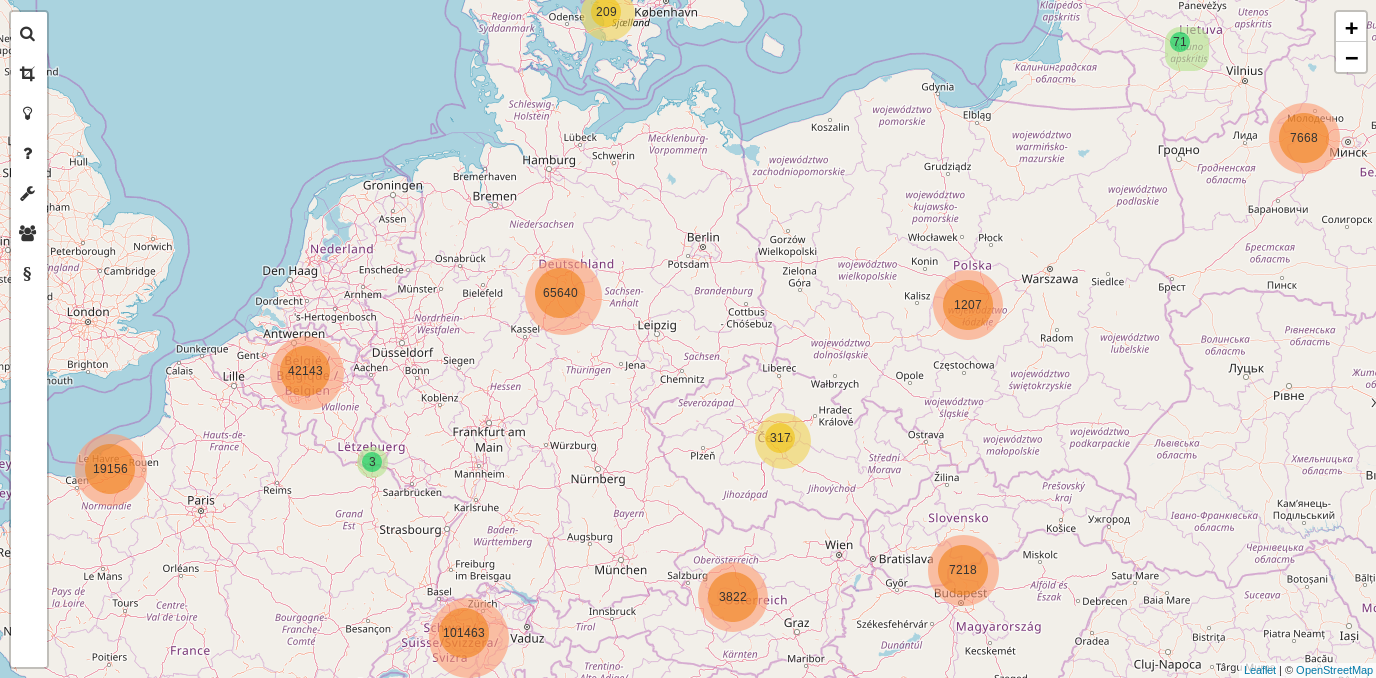
\includegraphics[height=0.5\textheight]{images/oscar}
		\caption{OpenStreetMap basierte Suchmaschine OSCAR \cite{oscar}}
	\end{figure}
\end{frame}

\begin{frame}{Problemstellung}
	viele nicht intuitive Tags:
	\begin{exampleblock}{}
		\begin{itemize}
			\item Tag:man\_made=beacon
			\item Tag:service=siding
			\item Tag:leisure=bird\_hide
			\item Tag:entrance=exit
			\item ...
		\end{itemize}
	\end{exampleblock}
\end{frame}

\section{Lösung}
\subsection{Datengrundlage schaffen}
\begin{frame}{Datengrundlage schaffen}
\begin{figure}[ht]
\begin{minipage}{0.44\linewidth}
	\begin{figure}
		
\includegraphics[width=\textwidth]{images/Openstreetmap_logo}
		\caption{OpenstreetMap-Wiki \cite{osmwiki}}
		\label{fig:openstreetmaplogo}
	\end{figure}
\end{minipage}
\hspace{0.5cm}
\begin{minipage}{0.44\linewidth}
	\begin{figure}
		
\includegraphics[width=\textwidth]{images/taginfo}
		\caption{TagInfo-Database \cite{taginfo}}
		\label{fig:taginfo}
	\end{figure}
\end{minipage}
\end{figure}
\end{frame}

\subsection{Daten aufbereiten}
\begin{frame}{Daten aufbereiten}
	\begin{exampleblock}{Urls}
		\begin{itemize}
			\item \textbf<2>{wiki.openstreetmap.org/wiki/Tag:highway=motorway}
			\item \textbf<2>{wiki.openstreetmap.org/wiki/Tag:waterway=canal}
			\item \textbf<2>{wiki.openstreetmap.org/wiki/Tag:highway=residential}
			\item \sout<2>{wiki.openstreetmap.org/wiki/Key:highway}
			\item \sout<2>{wiki.openstreetmap.org/wiki/Key:motorroad}
			\item \sout<2>{wiki.openstreetmap.org/wiki/Contributors}
		\end{itemize}
	\end{exampleblock}
\end{frame}


\begin{frame}{Daten aufbereiten}
\begin{figure}[!ht]
	\centering
\begin{tikzpicture}
\node (html) {
\includegraphics[width=4cm]{images/scrapy}};
\node (urls) [below=of html] {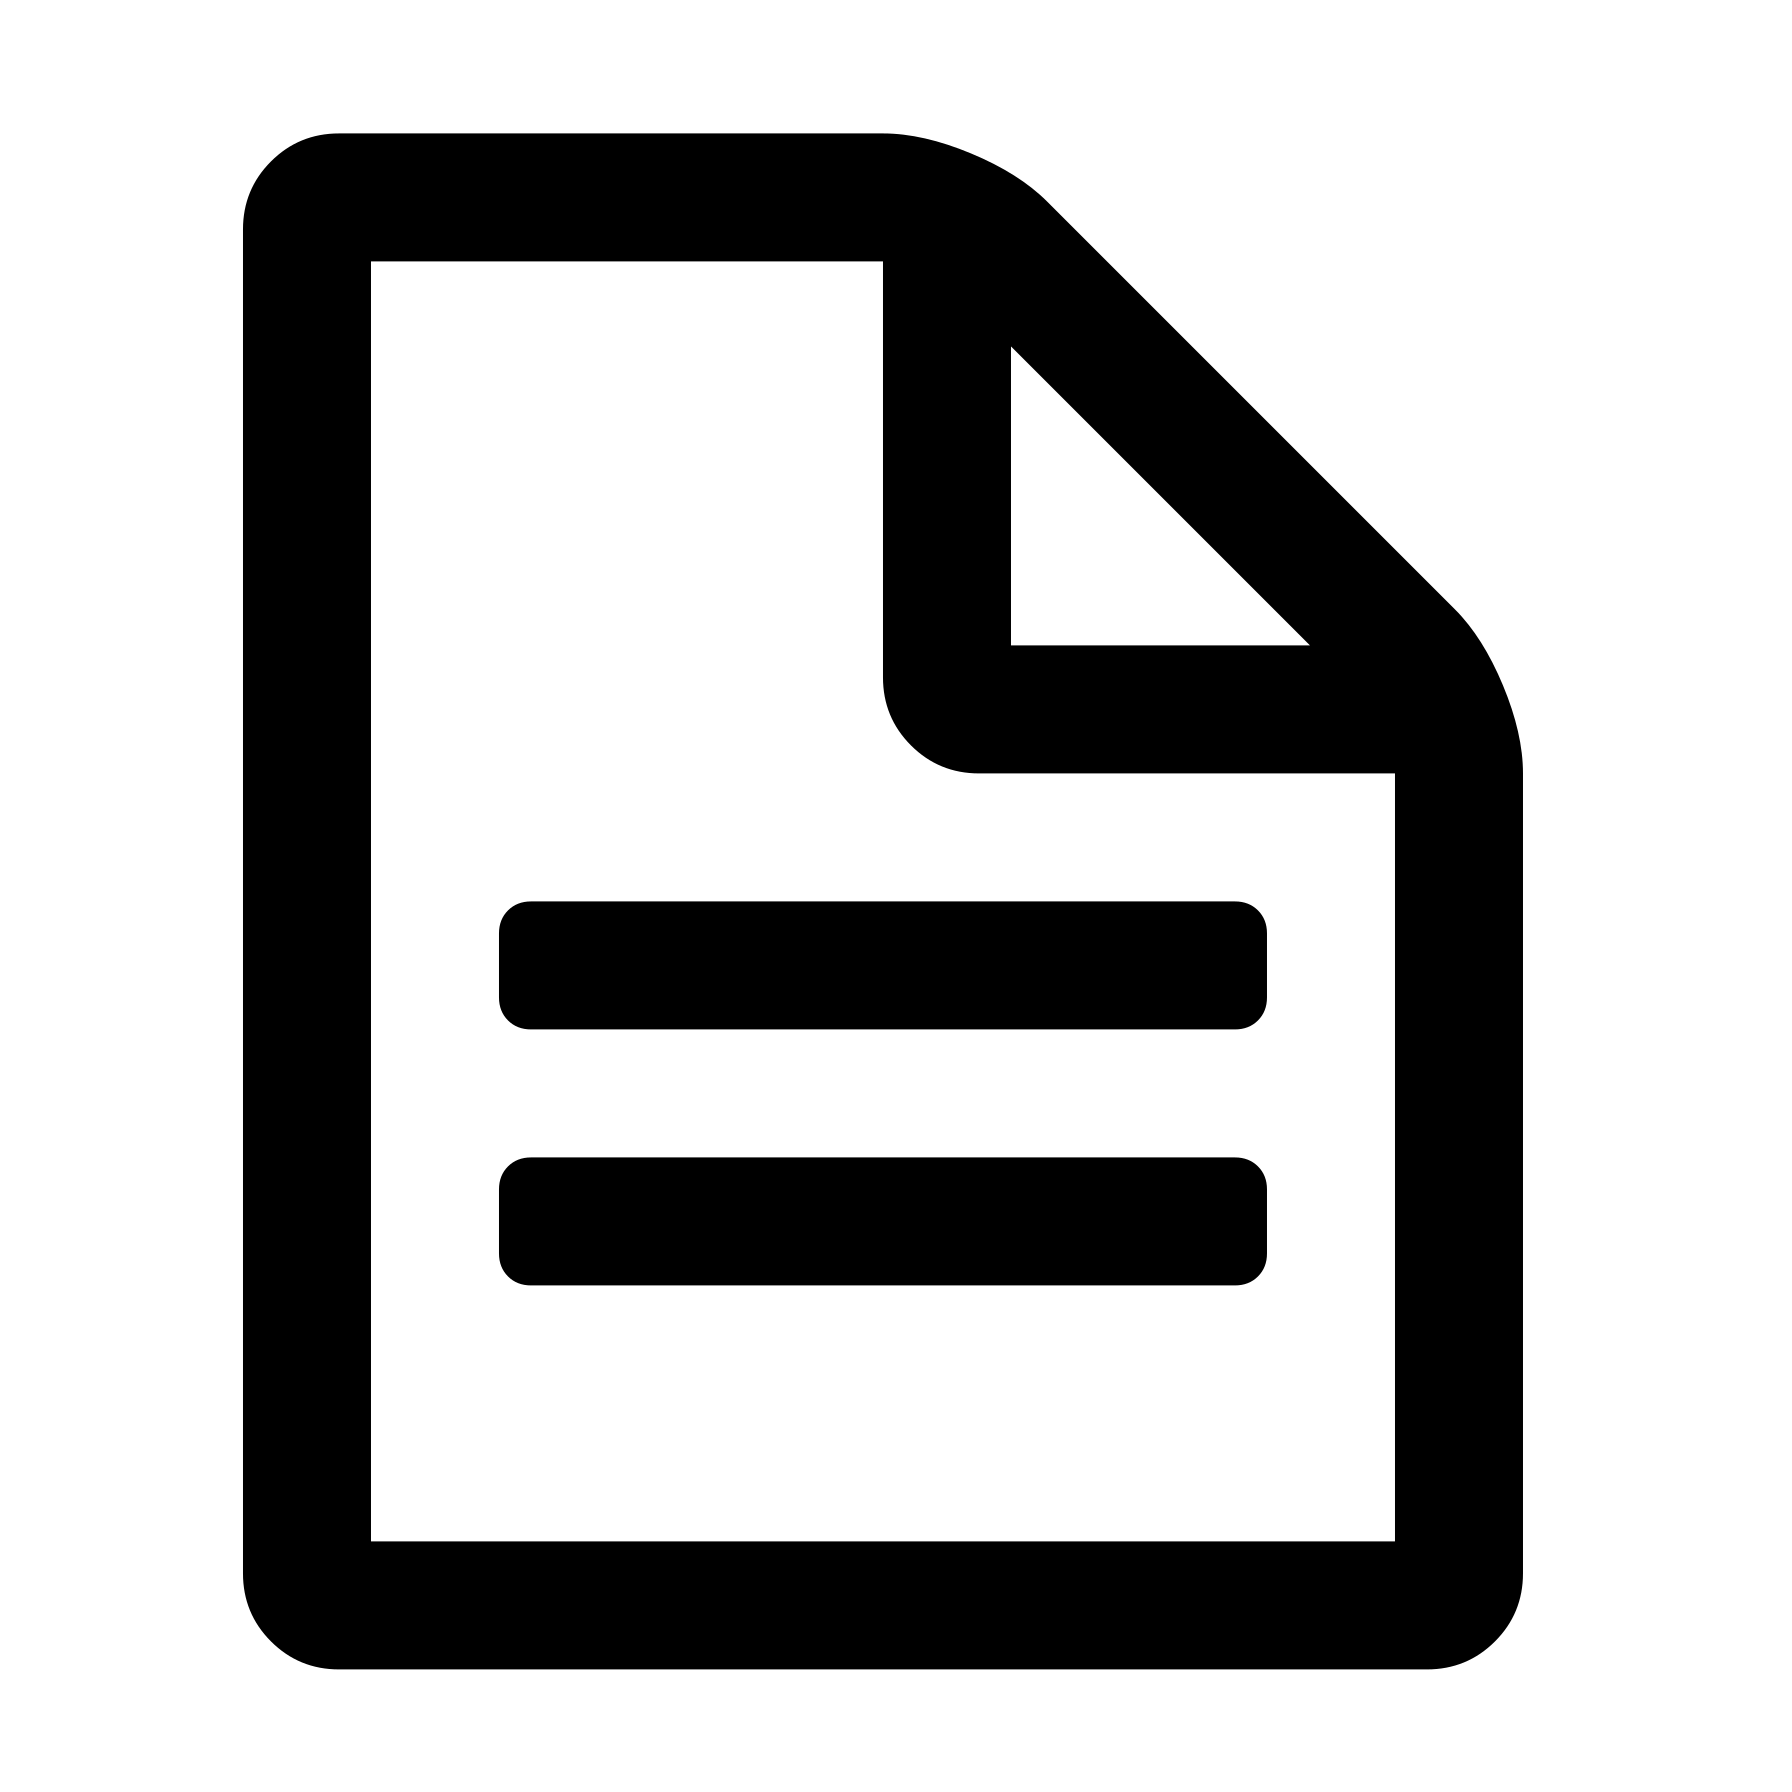
\includegraphics[height=2cm]{images/file}};
\node (objects) [right=of html] {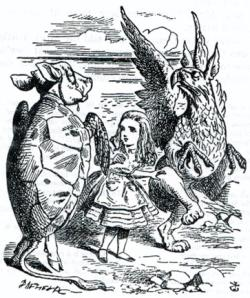
\includegraphics[height=2cm]{images/beautiful_soup}};
\node (json) [below=of objects] {
\includegraphics[height=2cm]{images/json}};

\node (a) [fill=white!1,draw, below of=urls] {URLS};
\node (b) [fill=white!1,draw, above of=objects] {Beatuiful Soup};
\node (b) [fill=white!1,draw, below of=json] {JSON};

\draw [ultra thick,orange,->] (html) to (objects);
\draw [ultra thick,orange,->] (urls) to (html);
\draw [ultra thick,orange,->] (objects) to (json);
\end{tikzpicture}
\end{figure}
\end{frame}

\begin{frame}{Daten}
\begin{figure}[!ht]
	\begin{minipage}{0.45\linewidth}
		\begin{figure}
			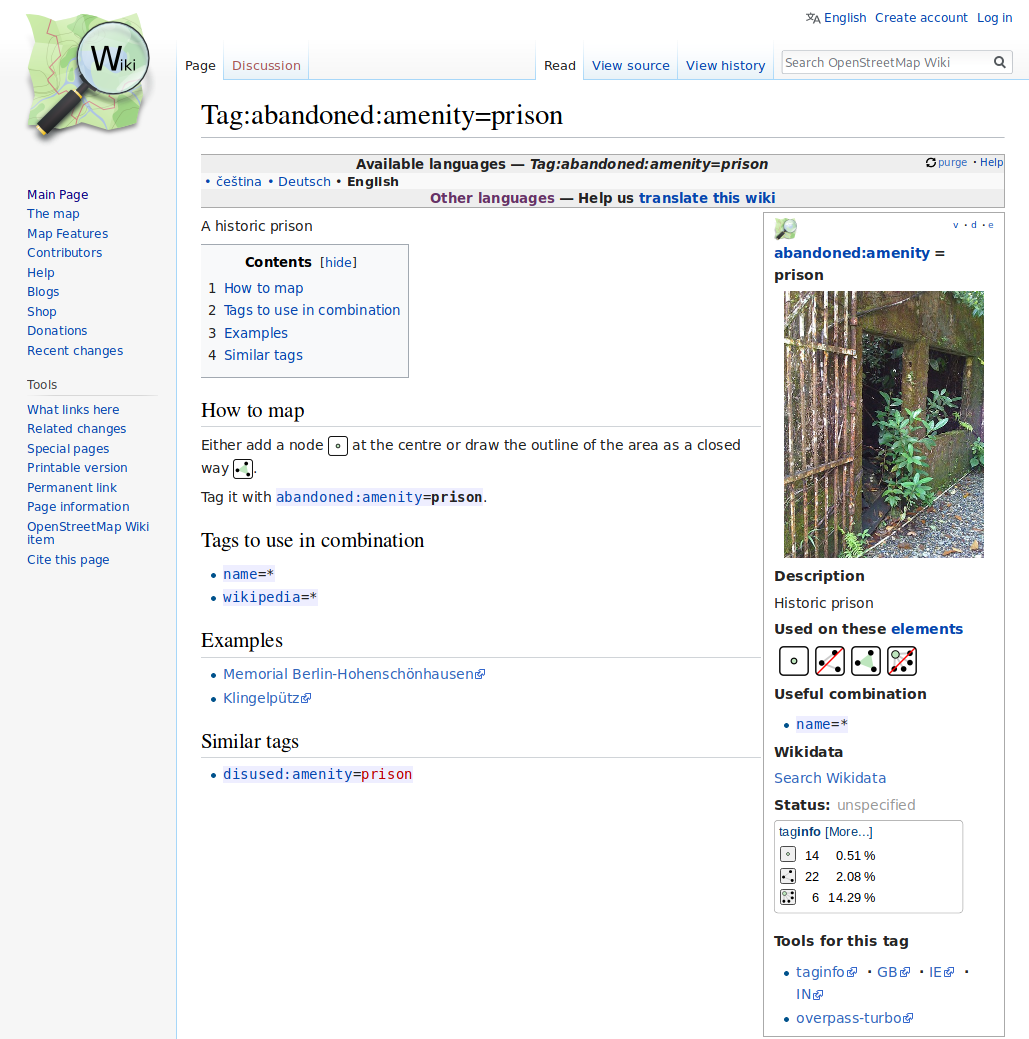
\includegraphics[width=\textwidth]{images/wiki}
			\label{fig:openstreetmaplogo}
			\caption{Wiki Example}
		\end{figure}
	\end{minipage}
	\hspace{0.5cm}
	\begin{minipage}{0.45\linewidth}
		\begin{figure}
			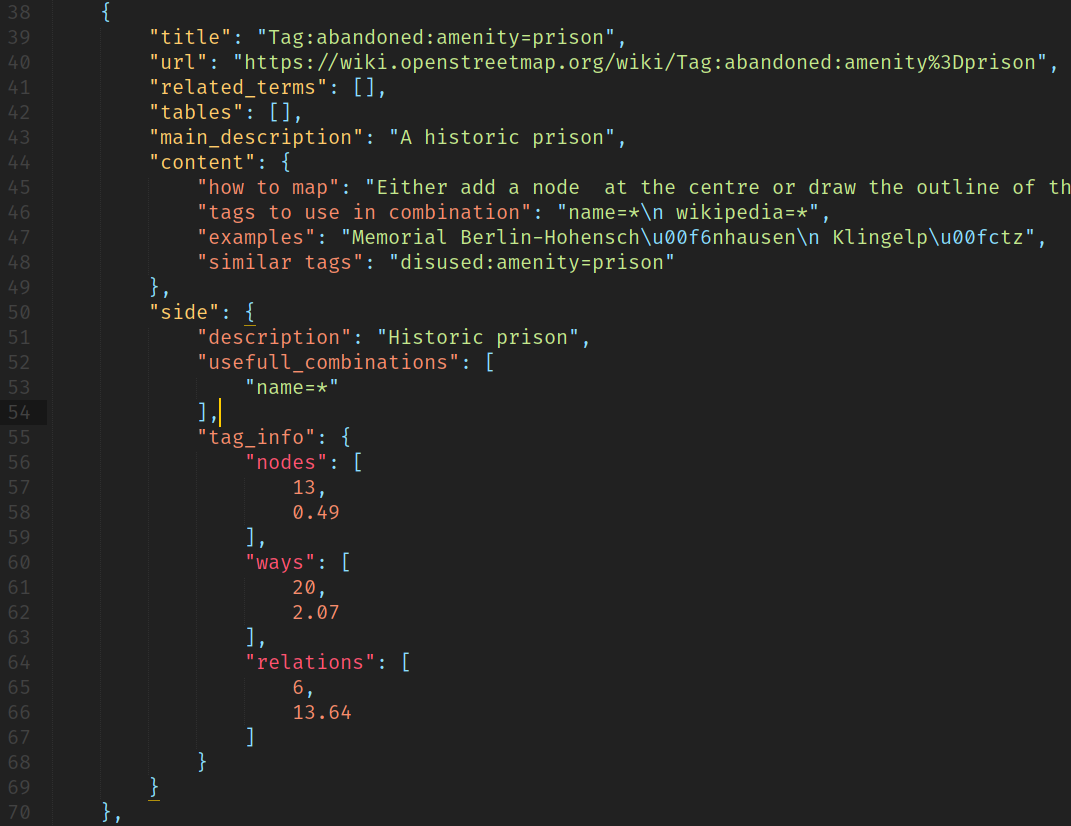
\includegraphics[width=\textwidth]{images/jsonexample}
			\label{fig:taginfo}
			\caption{Json Example}
		\end{figure}
	\end{minipage}
\end{figure}
\end{frame}

\subsection{Architektur}
\begin{frame}{Architektur}
	\begin{figure}
		\hspace*{-\beamerleftmargin}%
		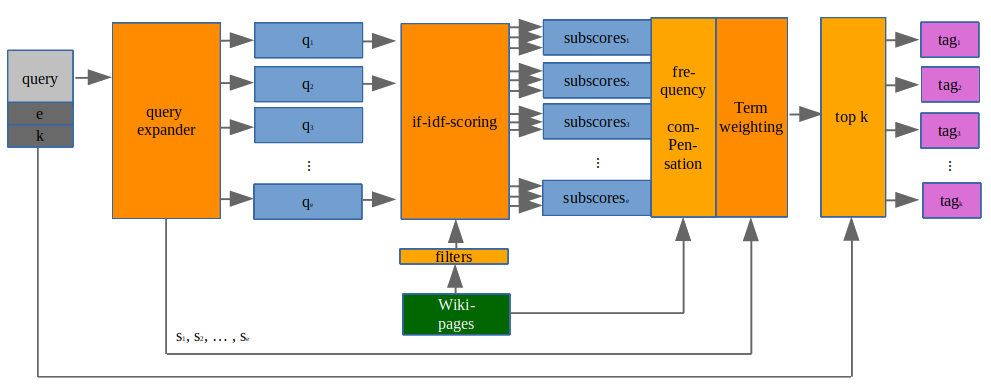
\includegraphics[width=\paperwidth,width=\paperwidth]{images/structure}
		\caption{Architektur}
		\centering
	\end{figure}
\end{frame}

\section{Demo}


\section{Verbesserungsmöglichkeiten}
\begin{frame}{Verbesserungsmöglichkeiten}
\begin{alertblock}{}
	\begin{itemize}
		\item Google Word2Vec-Model verkleinerns
		\item Syntaktische um Semantische Suche ergänzen
		\item Struktur besser ausnutzen
		\item Eingabekorrektur
	\end{itemize}
\end{alertblock}
\end{frame}



\appendix
\begin{frame}[allowframebreaks]{Quellen}
	\bibliography{presentation}
	\bibliographystyle{abbrv}
\end{frame}

\begin{frame}[standout]
	Vielen Dank für Ihre Aufmerksamkeit!\\~\\
	Gibt es Fragen?
\end{frame}

\end{document}